\subsection{Problems with Runtime Variability}

\begin{frame}{Recap: How to Implement Software Product Lines?}
	\begin{mycolumns}[widths={45},animation=none]
		
\includegraphics[width=\linewidth]{metaproduct2}	
	\mynextcolumn
		\mynote{Key Issues}{
			\begin{itemize}
			\item Systematic reuse of implementation artifacts.
			\item Explicit handling of variability.
			\end{itemize}
		}
		\uncover<2->{\mydefinition{Variability\mysource{\fospl\mypage{48}}}{
			Variability is the ability to derive different products from a common set of artifacts.
		}}
		\uncover<3->{\mynote{}{
			Any software product line is a variability-intensive system.
		}}
	\end{mycolumns}
\end{frame}

\begin{frame}{Recap: Variability and Binding Times}
	\begin{mycolumns}[widths={45},animation=none]
		
\includegraphics[width=\linewidth]{metaproduct2}	
	\mynextcolumn
		\mydefinition{Binding Time}{
			\begin{itemize}
				\item Variability offers choices.
				\item Derivation of a product requires to make decisions (aka. binding).
				\item Decisions may be bound at different binding times.
			\end{itemize}
		}	
		
		~
		
		\uncover<2->{\mynote{}{
			When, how and by whom?
		}}
	\end{mycolumns}
\end{frame}

\begin{frame}{Recap: Runtime Variability}
	\begin{mycolumns}[widths={45},animation=keep]
		\mynote{Basic Principles}{
			{\bf Configuration/Runtime Parameters:}
			\begin{itemize}
				\item Conditional statements controlled by configuration parameters
				\item Global variables vs.\ method parameter passing
			\end{itemize}	
			\vspace{2mm}
			{\bf Object-Orientation and Design Patterns:}
			\begin{itemize}
				\item Template Method
				\item Abstract Factory
				\item Decorator
				\item etc.
			\end{itemize}	
		}
	\mynextcolumn
		\mynote{Problems}{
			{\bf Conditional Statements:}
			\begin{itemize}
				\item Code scattering, tangling, and replication.
			\end{itemize}	
			\vspace{2mm}
			{\bf Design Patterns for Variability:}
			\begin{itemize}
				\item Trade-offs and potential negative side effects.
				\item Constraints that may restrict their usage.
			\end{itemize}	
			\vspace{2mm}
			{\bf More generally:}
			\begin{itemize}
				\item Variable parts are always delivered.
				\item Not well-suited for compile-time binding.
			\end{itemize}	
		}	
	\end{mycolumns}	
\end{frame}

\subsection{Compile-Time Variability}

\begin{frame}{\myframetitle}
	\begin{mycolumns}[columns=2,widths={40,60},animation=none]
		\mynote{Problems with Runtime Variability}{	
			{\bf Conditional Statements:}
			\begin{itemize}
				\item Code scattering, tangling, and replication.
			\end{itemize}	
			{\bf Design Patterns for Variability:}
			\begin{itemize}
				\item Trade-offs and potential negative side effects.
				\item Constraints that may restrict their usage.
			\end{itemize}	
			{\bf More generally:}
			\begin{itemize}
				\item Variable parts are always delivered.
				\item Not well-suited for compile-time binding.
			\end{itemize}	
		}			
	\mynextcolumn
		\uncover<2->{\mydefinition{Compile-Time Variability\mysource{\fospl\mypage{49}}}{
			Compile-time variability is decided before or at compile time.
		}}	
		\uncover<3->{\mynote{}{
			{\bf Goals:}
			\begin{itemize}
				\item Only required source code is compiled.
				\item Smaller and highly optimized variants.
			\end{itemize}				
			{\bf Challenge:}
			\begin{itemize}
				\item How to implement options and alternatives (i.e., variability)?
			\end{itemize}	
		}}
		\uncover<4->{\mynote{In This Lecture}{
			Simple concepts and techniques for a few variants.
		}}
	\end{mycolumns}	
\end{frame}

\subsection{Ad-Hoc/Unmanaged Clone-and-Own}

\begin{frame}{Ad-Hoc/Unmanaged Clown-and-Own}
	\begin{mycolumns}[columns=2,widths={50,50},animation=none]
		\mydefinition{Clown-and-Own}{	
			\begin{itemize}
				\item New variants of a software system are created by copying and adapting an existing variant.
				\item Afterwards, cloned variants evolve independently of each other.
			\end{itemize}	
		}	
		\vspace{3mm}		
		\myexample{Cloning Whole Products (Clone-and-Own)}{~\hfill
\includegraphics[width=.2\linewidth]{130}\hfill
\includegraphics[width=.2\linewidth]{230}\hfill~}
	\mynextcolumn
		\pic[width=\linewidth,page=24]{lego}
	\end{mycolumns}	
\end{frame}

\begin{frame}[fragile]{Example: Ad-Hoc Clone-and-Own}
	\vspace{-1.2cm}
	\begin{flushright}
		\includegraphics[scale=0.3,page=6]{graphs}		
	\end{flushright}
	\vspace{0.1cm}
	\begin{tiny}
		\begin{columns}
			\column{.45\textwidth}
				\vspace{-15mm}
				\mynote{}{
					\normalsize
					An initial implementation of our graph library providing weighted graphs.
				}
\vspace{3mm}				
\begin{codetight}{}
public class Graph {
	List nodes = new ArrayList();
	List edges = new ArrayList();

	Edge add(Node n, Node m) {
		Edge e = new Edge(n, m);
		nodes.add(n); nodes.add(m); edges.add(e);
		e.weight = new Weight();
		return e;
	}
	Edge add(Node n, Node m, Weight w) {
		Edge e = new Edge(n, m);
		nodes.add(n); nodes.add(m); edges.add(e);
		e.weight = w;
		return e;
	}
	void print() {
		for (int i = 0; i < edges.size(); i++) {
			((Edge) edges.get(i)).print();
		}
	}
}
\end{codetight}
			\column{.45\textwidth}
\begin{codetight}{}
public class Edge {
	Node a, b;
	Weight weight = new Weight();

	Edge(Node _a, Node _b) {
		a = _a; b = _b;
	}
	void print() {
		a.print(); b.print();
		weight.print();
	}
}
\end{codetight}
\begin{codetight}{}
public class Weight {
	void print() {...}
}
\end{codetight}
		\end{columns}
	\end{tiny}
\end{frame}

\begin{frame}[fragile]{Alice's Clone: Unweighted Graphs}
	\vspace{-1.2cm}
	\begin{flushright}
		
\includegraphics[scale=0.3]{alice}
		\includegraphics[scale=0.3,page=2]{graphs}
	\end{flushright}
	\begin{tiny}
		\begin{columns}
			\column{.45\textwidth}
				\vspace{-15mm}				
				\mynote{}{
					\normalsize
					Alice works with unweighted graphs, so she copies and adapts the basic implementation.
				}
\vspace{3mm}
\begin{codetight}{}
public class Graph {
	List nodes = new ArrayList();
	List edges = new ArrayList();

	Edge add(Node n, Node m) {
		Edge e = new Edge(n, m);
		nodes.add(n); nodes.add(m); edges.add(e);
		@|e.weight = new Weight();|@
		return e;
	}
	@|Edge add(Node n, Node m, Weight w) {
		Edge e = new Edge(n, m);
		nodes.add(n); nodes.add(m); edges.add(e);
		e.weight = w;
		return e;
	}|@
	void print() {
		for (int i = 0; i < edges.size(); i++) {
			((Edge) edges.get(i)).print();
		}
	}
}
\end{codetight}
			\column{.45\textwidth}
\begin{codetight}{}
public class Edge {
	Node a, b;
	@|Weight weight = new Weight();|@

	Edge(Node _a, Node _b) {
		a = _a; b = _b;
	}
	void print() {
		a.print(); b.print();
		@|weight.print();|@
	}
}
\end{codetight}
\begin{codetight}{}
@|public class Weight {
	void print() {...}
}|@
\end{codetight}
		\end{columns}
	\end{tiny}
\end{frame}

\begin{frame}[fragile]{Alice's Clone: Unweighted Graphs}
	\vspace{-1.5cm}
	\begin{flushright}
		
\includegraphics[scale=0.3]{alice}
		\includegraphics[scale=0.3,page=2]{graphs}
	\end{flushright}
	\begin{tiny}
		\begin{columns}
			\column{.45\textwidth}
				\vspace{-3mm}				
				\mynote{}{
					\normalsize
					Alice works with unweighted graphs, so she copies and adapts the basic implementation.
				}
\vspace{3mm}
\begin{codetight}{}
public class Graph {
	List nodes = new ArrayList();
	List edges = new ArrayList();

	Edge add(Node n, Node m) {
		Edge e = new Edge(n, m);
		nodes.add(n); nodes.add(m); edges.add(e);
		return e;
	}
	void print() {
		for (int i = 0; i < edges.size(); i++) {
			((Edge) edges.get(i)).print();
		}
	}
}
\end{codetight}
			\column{.45\textwidth}
\begin{codetight}{}
public class Node {
	int id = 0;

	void print() {
		System.out.print(id);
	}
}
\end{codetight}
\begin{codetight}{}
public class Edge {
	Node a, b;

	Edge(Node _a, Node _b) {
		a = _a; b = _b;
	}
	void print() {
		a.print(); b.print();
	}
}
\end{codetight}
		\end{columns}
	\end{tiny}
\end{frame}

\begin{frame}[fragile]{Bob's Clone: Colored Graphs}
	\vspace{-1.6cm}
	\begin{flushright}
		
\includegraphics[scale=0.3]{bob}
		\includegraphics[scale=0.3,page=12]{graphs}
	\end{flushright}
	\vspace{0.1cm}
	\begin{tiny}
		\begin{columns}
			\column{.45\textwidth}
				\vspace{-10mm}
				\mynote{}{
					\normalsize
					Bob works with colored (unweighted) graphs. He is a colleague of Alice and knows her variant, so he copies and adapts Alice's variant.
				}
\vspace{3mm}					
\begin{codetight}{}
public class Graph {
	List nodes = new ArrayList();
	List edges = new ArrayList();

	Edge add(Node n, Node m) {
		Edge e = new Edge(n, m);
		nodes.add(n); nodes.add(m); edges.add(e);
		return e;
	}
	void print() {
		for (int i = 0; i < edges.size(); i++) {
			((Edge) edges.get(i)).print();
		}
	}
}
\end{codetight}	
			\column{.45\textwidth}
\begin{codetight}{}
public class Node {
	int id = 0;
	~Color color = new Color();~

	void print() {
		~Color.setDisplayColor(color);~
		System.out.print(id);
	}
}
\end{codetight}
\begin{codetight}{}
~public class Color {
	static void setDisplayColor(Color c) {...}
}~
\end{codetight}
		\end{columns}
	\end{tiny}
\end{frame}

\subsection{Problems and Discussion}

\begin{frame}{Problem: Feature Combinations}
	\vspace{-1.2cm}
	\begin{flushright}
		
\includegraphics[scale=0.3]{eve}
		\includegraphics[scale=0.3,page=16]{graphs}
	\end{flushright}	
	\begin{columns}
		\column{.55\textwidth}			
			\vspace{-1.3cm}
			\mynote{}{				
				Eve has a new requirement:
				She wants to work with graphs which are both colored and weighted.
			}
			\vspace{2mm}
			\mynote{}{				
				\begin{itemize}
					\item Where to start from? 
					\item Does Eve know about Bob's and Alice's variants?
					\item If so, how to avoid repeating the work that has been already done by Alice and Bob, respectively?
				\end{itemize}
			}
		\column{.4\textwidth}			
			~
	\end{columns}	
	\vspace{5mm}
	\includegraphics[scale=0.3,page=6]{graphs}
	\hspace{5mm}
	
\includegraphics[scale=0.3]{alice}
	\includegraphics[scale=0.3,page=2]{graphs}
	\hspace{5mm}
	
\includegraphics[scale=0.3]{bob}
	\includegraphics[scale=0.3,page=12]{graphs}
\end{frame}

\begin{frame}[fragile]{Problem: Evolution and Maintenance}
	\vspace{-1.7cm}
	\begin{flushright}		
		\includegraphics[scale=0.3,page=6]{graphs}
	\end{flushright}
	\vspace{0.1cm}
	\begin{tiny}
		\begin{columns}
			\column{.45\textwidth}
				\vspace{-12mm}
				\mynote{}{
					\normalsize
					Maintainers of the initial variant refactor the code of the basic implementation.
				}
\vspace{3mm}					
\begin{codetight}{}
public class Graph {
	...
	Edge add(Node n, Node m) {
		Edge e = new Edge(n, m);
		nodes.add(n); nodes.add(m); edges.add(e);
		e.weight = new Weight();
		return e;
	}
	Edge add(Node n, Node m, Weight w) {
		@|Edge e = new Edge(n, m);|@
		@|nodes.add(n); nodes.add(m); edges.add(e);|@
		?Edge e = this(n, m);?	
		e.weight = w;
		return e;
	}
	...
}
\end{codetight}	
			\column{.45\textwidth}
				\mynote{}{
					\normalsize
					\begin{itemize}
						\item Who informs Alice, Bob and Eve about the improvement?
						\item How do they know whether the improvement is relevant for them?
						\item If so, how to propagate the improvement to their variant?
					\end{itemize}									
				}
				\vspace{2mm}
				
\includegraphics[scale=0.1]{alice}
				\includegraphics[scale=0.13,page=2]{graphs}
				\hspace{2.5mm}
				
\includegraphics[scale=0.1]{bob}
				\includegraphics[scale=0.13,page=12]{graphs}
				\hspace{2.5mm}
				
\includegraphics[scale=0.1]{eve}
				\includegraphics[scale=0.13,page=16]{graphs}
		\end{columns}
	\end{tiny}
\end{frame}

\begin{frame}{Discussion}
	\begin{mycolumns}[columns=2,widths={45,55},animation=none]
		\mynote{Advantages}{	
			\begin{itemize}
				\item Simple and straightforward approach.
				\item Rapid exploration of new ideas.
				\item No upfront investments.	
			\end{itemize}
		}
	\mynextcolumn
		\mynote{Disadvantages}{	
			\begin{itemize}
				\item No structured and systematic reuse (copy \& edit).
				\item No flexible combination of features.
				\item Maintenance quickly becomes impractical.	
			\end{itemize}			
		}	
	\end{mycolumns}	
		\uncover<2->{\mynote{Towards Managed Clone-and-Own}{	
			\begin{itemize}
				\item How can we better manage such clone-and-own development?
				\item The traditional answer: Software Configuration Management
				\item In the sequel: Software Configuration Management in practice.
			\end{itemize}
		}}
\end{frame}